\documentclass[12pt, a4paper]{report}
\usepackage{graphicx, array, amsthm, amssymb, amsmath, algorithm, algpseudocode, float, xcolor, thmtools, thmbox}
\usepackage[english]{babel}

\makeatletter
\renewcommand\thmbox@headstyle[2]{\bfseries #1}
\makeatother
\newtheorem[style=M,bodystyle=\normalfont]{theorem}{Theorem}
\newtheorem[style=M,bodystyle=\normalfont]{corollary}{Corollary}
\newtheorem[style=M,bodystyle=\normalfont]{lemma}{Lemma}
\newtheorem[style=M,bodystyle=\normalfont]{definition}{Definition}


\title{Numerical Analysis \\ \textit{Theory}}
\author{Christian Rossi}
\date{Academic Year 2023-2024}

\begin{document}

\maketitle

\newpage

\begin{abstract}
The topics of the course are:
\begin{itemize}
    \item Floating-point arithmetic: different sources of the computational error; absolute vs relative errors; the floating point representation 
        of real numbers; the round-off unit; the machine epsilon; floating-point operations; over- and under-flow; numerical cancellation.
    \item Numerical approximation of nonlinear equations: the bisection and the Newton methods; the fixed-point iteration; convergence analysis 
        (global and local results); order of convergence; stopping criteria and corresponding reliability; generalization to the system of 
        nonlinear equations (hints).
    \item Numerical approximation of systems of linear equations: direct methods (Gaussian elimination method; LU and Cholesky factorizations; 
        pivoting; sparse systems: Thomas algorithm for tridiagonal systems); iterative methods (the stationary and the dynamic Richardson scheme; 
        Jacobi, Gauss-Seidel, gradient, conjugate gradient methods (hints); choice of the preconditioner; stopping criteria and corresponding 
        reliability); accuracy and stability of the approximation; the condition number of a matrix; over- and under-determined systems: the 
        singular value decomposition (hints).
    \item Numerical approximation of functions and data: Polynomial interpolation (Lagrange form); piecewise interpolation; cubic interpolating 
        splines; least-squares approximation of clouds of data.
    \item Numerical approximation of derivatives: finite difference schemes of the first and second order; the undetermined coefficient method.
    \item Numerical approximation of definite integrals: simple and composite formulas; midpoint, trapezoidal, Cavalieri-Simpson quadrature rules; 
        Gaussian formulas; degree of exactness and order of accuracy of a quadrature rule. 
    \item Numerical approximation of ODEs: the Cauchy problem; one-step methods (forward and backward Euler and Crank-Nicolson schemes); 
        consistency, stability, and convergence (hints).
\end{itemize}
\end{abstract}

\newpage

\tableofcontents

\newpage

\chapter{Introduction}
\section{Numerical analysis and errors}
Numerical analysis is the field of mathematics dealing with methods to find the solutions of certain mathematical problems with an electronic 
calculator. It is the intersection between math and computer science. 

On the other hand, scientific computing also deals with the model formalization and so it needs also engineering knowledge. 
\begin{figure}[H]
    \centering
    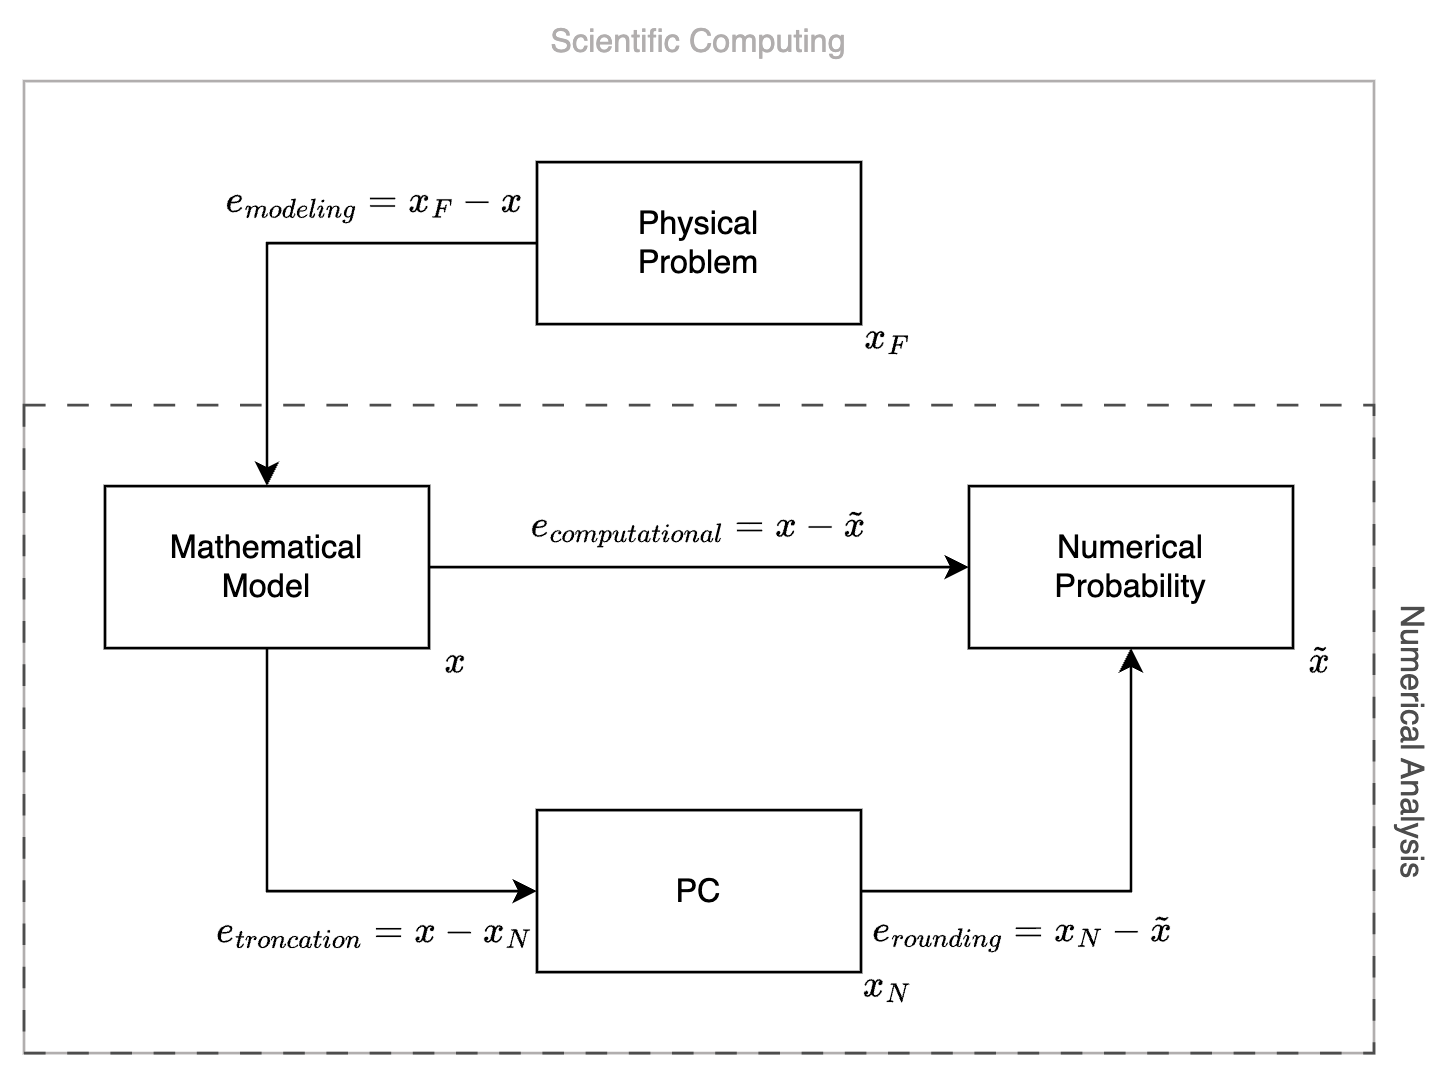
\includegraphics[width=0.75\linewidth]{images/difference.png}
    \caption{Difference between numerical analysis and scientific computing}
\end{figure}
As it is possible to see from the diagram every step of the computation have to deal with errors. The possible types of errors are: 
\begin{itemize}
    \item Absolute: $\left\lvert x - \tilde{x} \right\rvert$
    \item Relative: $\dfrac{\left\lvert x - \tilde{x} \right\rvert}{\left\lvert x \right\rvert}$, where $x \neq 0$
\end{itemize}
The relative error is more precise because it compares the error with the measure quantity. 
\begin{example}
    Let us consider $x=100$ and $\tilde{x}=100.1$. The errors in this case are: 
    \[e_{abs}=\left\lvert x - \tilde{x} \right\rvert=\left\lvert 100 - 100.1 \right\rvert=0.1\]
    \[e_{rel}=\dfrac{\left\lvert x - \tilde{x} \right\rvert}{\left\lvert x \right\rvert}=\dfrac{\left\lvert 100 - 100.1 \right\rvert}{\left\lvert 100 \right\rvert}=0.001\]
    Let us consider $x=0.2$ and $\tilde{x}=0.1$. The errors in this case are: 
    \[e_{abs}=\left\lvert x - \tilde{x} \right\rvert=\left\lvert 0.2 - 0.1 \right\rvert=0.1\]
    \[e_{rel}=\dfrac{\left\lvert x - \tilde{x} \right\rvert}{\left\lvert x \right\rvert}=\dfrac{\left\lvert 0.2 - 0.1 \right\rvert}{\left\lvert 0.2 \right\rvert}=0.5\]
    The result are that the measures have the same absolute error ($10\%$), but the relative error is much grater in the second example ($50\%$ vs $0.1\%$).
    This result proves that the relative error is the most precise.
\end{example}

\section{Floating point}
A calculator can only handle a finite quantity of numbers and compute a finite number of operations. For those reason the set of the real numbers 
$\mathbb{R}$ is indeed represented by a finite set of machine numbers $\mathbb{F}=\{-\tilde{a}_{min}, \dots , \tilde{a}_{max} \}$ called
floating points numbers. The function used to find the corresponding value in $\mathbb{F}$ to a number in $\mathbb{R}$ is $fl(x)$ that does an 
operation called truncation and rounding.

The set $\mathbb{F}=\mathbb{F}(\beta,t,L,U)$ is characterized by four parameters $\beta,t,L$ and $U$ such that every real number $fl(x) \in \mathbb{F}$ 
can be written as:
\[fl(x)=(-1)^sm\beta^{e-t}=(-1)^s(a_1a_2\dots a_t)_{\beta}\beta^{e-t}\]
where:
\begin{itemize}
    \item $\beta \geq 2$ is the basics, an integer that determines the numeric system. 
    \item $m=(a_1a_2\dots a_t)_{\beta}$ is the mantissa, $(0<m<\beta^t-1)$ where $t$ is the number of digits such that $0<a_1 \leq \beta - 1$
        and $0 \leq a_i \leq \beta - 1$ for $i=2, \dots, t$. 
    \item $e=\mathbb{Z}$ is the exponent such that $L<e<U$, with $L<0$ and $U>0$. 
    \item $s=\{0,1\}$ is the sign. 
\end{itemize}
In the definition of the numbers in the mantissa set we have to set the constraint $a_1 \neq 0$ to ensure the uniqueness of the representation. 

The set of floating points has the following characteristic values:
\begin{itemize}
    \item Machine epsilon, that is the distance between one and the smallest floating point number greater than one, and it is equal to: 
        \[\epsilon_M=\beta^{1-t}\]
    \item Round-off error, that is the relative error that is committed when substituting $x \in \mathbb{R}-\{0\}$ with his corresponding 
        $fl(x) \in \mathbb{F}$. It is limited by: 
        \[\dfrac{\left\lvert x-fl(x) \right\rvert}{\left\lvert x \right\rvert }\leq \dfrac{1}{2}\epsilon_M\]
        where $x \neq 0$.
    \item Cardinality of the floating point set:
        \[\#\mathbb{F}=2 \beta^{t-1}(\beta -1)(U-L+1)+1\]
        where: 
        \begin{itemize}
            \item $2$ is needed to consider both positive and negative numbers. 
            \item $\beta^{t-1}$ is the cardinality of values that can be taken by all digits.
            \item $(\beta -1)$ is the cardinality of values that can be taken by $a_1$.
            \item $(U-L+1)$ considers all the possible variations for the exponent.
            \item $1$ is needed to consider also the zero. 
        \end{itemize}
    \item The biggest and the smallest numbers in the set are found with the formula:
        \[x_{min}=\beta^{L-1}\]
        \[x_{max}=\beta^U(1-\beta^{-t})\]
\end{itemize}
\begin{example}
    In MATLAB the floating point set is defined with the following variables:
    \[(\beta=2,t=53,L=-1021,U=1024)\] 
    With the command $eps$ we can find the machine epsilon, that in MATLAB case is:
    \[\epsilon_M=2.22 \cdot 10^{-16}\]
    With the command $realmin$ and $realmax$ we can find the smallest and the largest numbers representable that are equal to:
    \[x_{min}=2.225073858507201 \cdot 10^{-308}\]
    \[x_{max}=1.797693134862316 \cdot 10^{308}\]
\end{example}
Since not all the numbers in the $\mathbb{R}$ set are also in the $\mathbb{F}$ set, in the second one there is no continuity. It is possible to 
demonstrate that while we are increasing the values of the numbers we are also increasing the distance between two consecutive numbers in $\mathbb{F}$.
\begin{example}
    Let us consider the floating number set $\mathbb{F}(2,2,-1,2)$. The characteristic values of this set are: 
    \begin{itemize}
        \item $\epsilon_M=\beta^{1-t}=0.5$.
        \item $x_{min}=\beta^{L-1}=0.25$.
        \item $x_{max}=\beta^U(1-\beta^t)=3$.
        \item $\#\mathbb{F}=2 \beta^{t-1}(\beta -1)(U-L+1)+1=16$. 
    \end{itemize}
    The exponent can have the values $-1,0,1$ and $2$. The mantissa will be like $(a_1a_2)_{\beta}$ because $t=2$. The possible positive values are
    reported in the figure. 
    \begin{figure}[H]
        \centering
        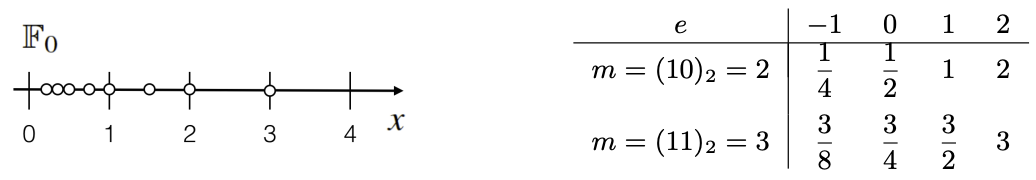
\includegraphics[width=0.9\linewidth]{images/numbers.png}
    \end{figure}
\end{example}
The other important aspect is that the passage between the two sets causes the loss of two important properties such as associativity end the 
neutral number for the sum. 



\end{document}